\section{Durchführung und Aufbau}
\label{sec:Durchführung}

Da die Energieunterschiede der Zeeman-Aufspaltung sehr gering ist, muss ein optisches Bauteil mit einem hohen Auflösungsvermögen verwendet werden. Dazu wird eine Lummer-Gehrcke-Platte verwendet, deren Funktionsweise im folgenden kurz skizziert wird. 
\subsection{Lummer-Gehrcke-Platte}
Bei einer Lummer-Gehrcke-Platte wird Licht durch ein durch ein Dreieckiges Prisma in zwei planparallele teildurchlässige Spiegel eingekoppelt. Das Licht wird an den Grenzflächen zu großem Teil reflektiert. Jedoch Tritt ein geringer Teil der Strahlung aus der Platte aus und interferiert mit den benachtbarten Strahlen welche immer genau im Abstand der Wellenlänge aus der Lummer-Gehrcke-Platte austreten. Ein Skizze der Lummer-Gehrcke-Platte ist in Abbildung \ref{fig:Lum} zu sehen.

\begin{figure}[H]
  \centering
  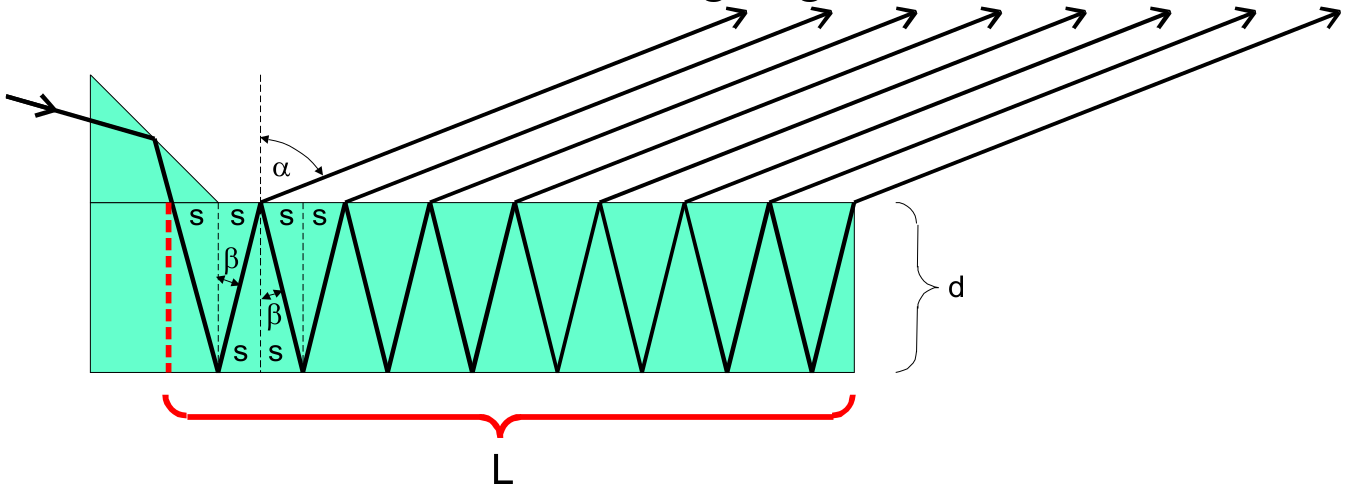
\includegraphics[height=6cm]{Bilder/Lummer.png}
  \caption{Funktionsweise einer Lummer-Gehrcke-Platte \cite{V27}}
  \label{fig:Lum}
\end{figure}

Die Strahelen interferieren Konstruktiv wenn sie die Gleichung 
\begin{equation}
  2 d \cos(\theta) = n \lambda
  \label{}
\end{equation}
erfüllen, wobei $d$ die Dicke der Platte ist.

\subsection{Versuchsaufbau}
Für den Versuch befindet sich zwischen den Polschuhen des Magneten eine Cd-Lampe dessen Strahl zunächst fokussiert und durch ein Gradsichprimsma geschickt wird. Anschließend wird das Licht durch eine Polarisationsfilter gelassen, welcher dazu dient den normalen vom annomalen Seemaneffekt unterscheiden zu können. Eine Linse wirft das Polarisierte Licht auf einen Spalt wodurch nur die gewünschte Farbe sich anschließend im Strahlengang befindet. 
\begin{figure}[H]
  \centering
  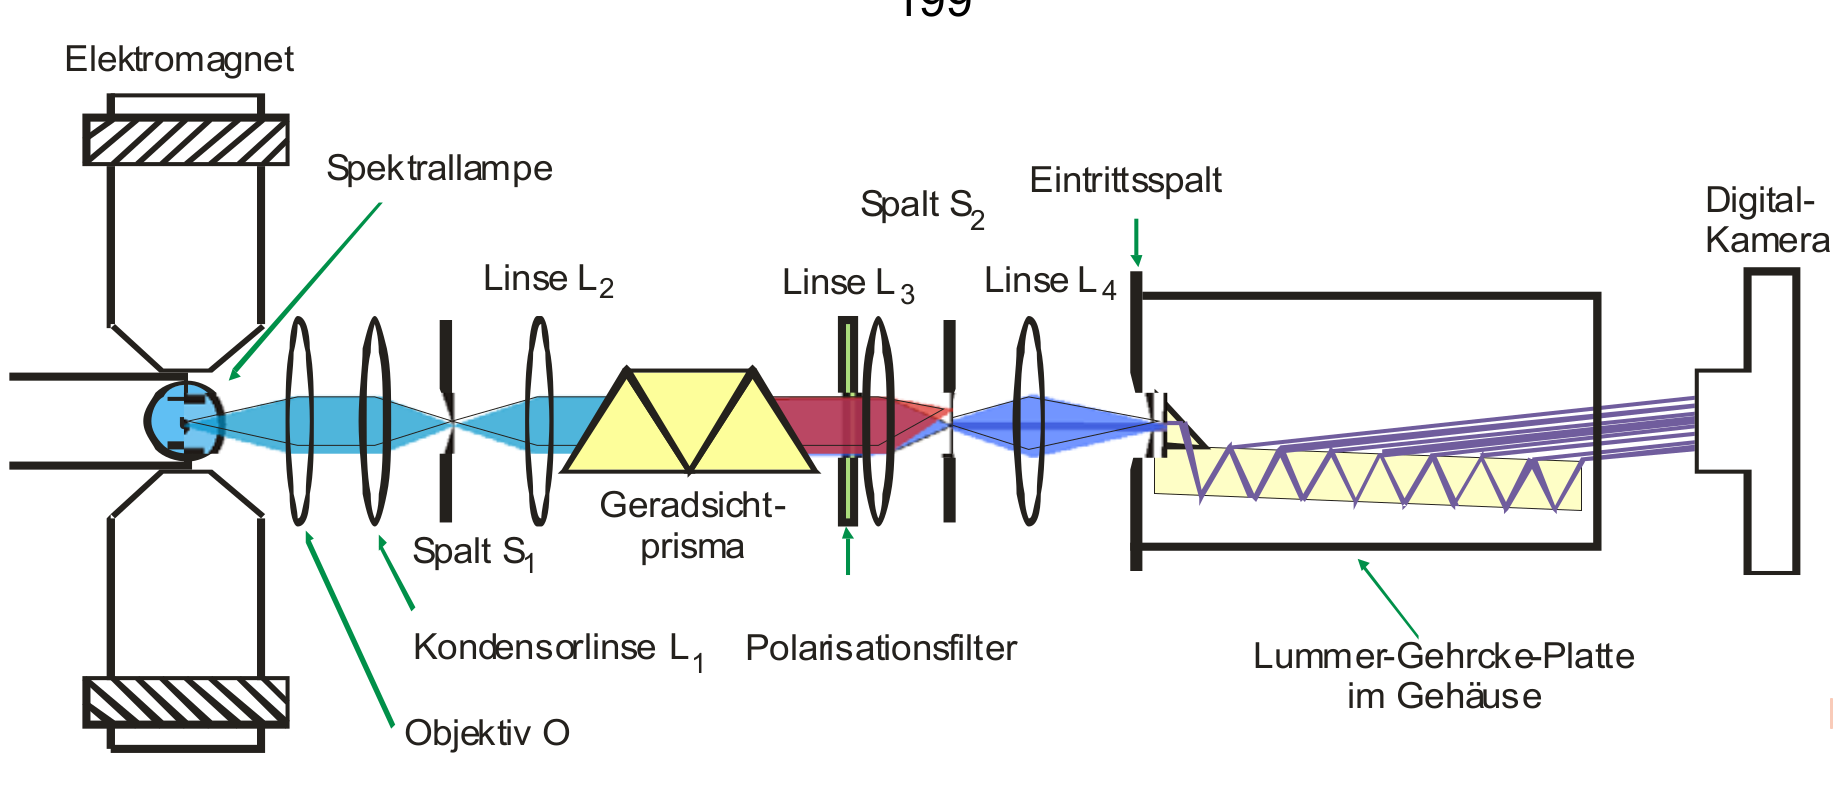
\includegraphics[height=6cm]{Bilder/Aufbau.png}
  \caption{Aufbau der Messaperatur \cite{V27}}
  \label{fig:<+label+>}
\end{figure}
Hinter dem Spalt wird eine weiter Linse aufgestellt um den Strahlengang auf die eintrittsöffnung der Lummer-Gehrcke-Platte scharf abzubilden. Zuletzt wird mittels einer Digitalkammera ein Foto von dem Beugungsbild geschossen.

\subsection{Durchführung}
Zuerst werden die optischen Bauteile in den Strahlengang gebracht und nacheinander ausgerichtet. Sofern dieses geschehen ist wird die Lummer-Gehrcke-Platte so ausgerichtet, dass das konstruktive Interferenzbild in der Kammera zu sehen ist. Dabei ist darauf zu achten das der Fokus der Kamer angepasst wird, damit das Bild scharf wird. Es wird jeweils zwei Bilder für die rote und Blaue Spektrallinie geschossen. Zunächst wird ein Bild der Spektrallinie ohne äußeres B-Feld und anschließend mit angelektem B-Feld ein Bild geschossen. Zuletzt wird eine Hysteresekurve des Magnetfeldes aufgenommen, wobei darauf zu achten ist, dass die Hallsonde möglichst nah an die Cd-Lampe zu halten ist um den Messfehler möglichst gering zu halten.
